\section{Results}
\label{sec:results}

\subsection{Three-pronged identification}
\label{subsec:three_pronged}

We identify the payment-friction--complex-trade mechanism using three reduced-form natural experiments. Each isolates a different source of variation in cross-border payment costs, and each delivers a coefficient on the friction--PCI interaction with the sign predicted by the model in Section~\ref{sec:strategy}. The three experiments differ in cleanliness, sign, and scope; together they form a tight causal triangle.

The first prong is the FATF greylist. Greylisting is a binary, country-level designation announced after a multi-year compliance review by the Financial Action Task Force, and the timing is exogenous to bilateral trade in goods. Greylisting raises correspondent-banking and KYC costs in affected corridors, predicting a negative coefficient on $\text{FATF}_{ct} \times \text{PCI}_p$. The second prong is the EU Anti-Money-Laundering Directive (AMLD4), effective in 2017, which harmonized KYC and AML standards across EU member states. Because complex products pass through more compliance gates per shipment, regulatory harmonization reduces friction differentially in EU corridors and predicts a \emph{positive} interaction coefficient. The third prong is the FDI-derisked corridor measure used in Section~\ref{sec:data}, which captures persistent corridor-level reductions in financial linkage and serves as the broad reduced form. Tables~\ref{tab:yearly_three_pronged} and~\ref{tab:panel_three_pronged} report the yearly cross-sections and the panel specifications respectively, and Figure~\ref{fig:confounder_compare} plots all three against one another.

\subsection{FATF greylist: the cleanest friction-up shock}
\label{subsec:fatf}

Table~\ref{tab:yearly_three_pronged}, Panel A reports year-by-year PPML cross-sections of the interaction $\text{FATF}_{ct} \times \text{PCI}_p$. The coefficient is negative in every year from 2018 to 2023. Point estimates range from $-0.354$ in 2018 to $-0.115$ in 2021, all six significant at the 1\% level. The two weakest-magnitude years, 2021 and 2023, coincide with COVID-related disruptions to the FATF review calendar.

The panel pair-fixed-effects specification (Table~\ref{tab:panel_three_pronged}, column~3) yields $\hat{\gamma}_{\text{FATF}} = -0.108$ ($p = 0.098$). The attenuation relative to the cross-sections is expected: pair fixed effects absorb time-invariant corridor characteristics that contribute to between-corridor variation. The coefficient survives this absorption.

Economic magnitude: a one-standard-deviation increase in product complexity reduces trade flow by $\exp(-0.108) - 1 = 10.2\%$ in greylisted corridors relative to non-greylisted corridors. This is the cleanest causal estimate in the paper. FATF designations follow a structured review process keyed to AML/CFT compliance \citep{Borchert2024_broken_relationships}, and the assignment is unrelated to bilateral trade in goods.

\subsection{EU AMLD: the symmetric friction-down shock}
\label{subsec:amld}

If payment frictions reduce complex trade, regulatory harmonization that lowers frictions raises it. AMLD4 provides such a shock. The directive imposed common KYC and AML standards across EU member states starting in 2017, reducing the per-corridor compliance burden disproportionately for products passing through more gates per shipment.

Table~\ref{tab:yearly_three_pronged}, Panel B reports the yearly interaction $\text{EU\_post2017}_{ct} \times \text{PCI}_p$. The coefficient is positive and significant at the 1\% level in every year from 2018 to 2023, ranging from $+0.096$ in 2022 to $+0.139$ in 2023. The panel specification (Table~\ref{tab:panel_three_pronged}, column~2) yields $\hat{\gamma}_{\text{AMLD}} = +0.141$ ($p = 0.040$).

Economic magnitude: a one-standard-deviation increase in PCI raises trade flow by $\exp(0.141) - 1 = 15.1\%$ in EU post-AMLD corridors. The sign is the mirror image of FATF. Friction up hurts complex trade; friction down helps it. Same mechanism, opposite sign.

We address two alternative interpretations. First, the AMLD coefficient may reflect rerouting: complex trade rerouted into EU corridors as non-EU corridors got greylisted. The triple horse race in Section~\ref{subsec:horserace} controls directly for FATF exposure, and the AMLD coefficient is preserved. Second, the post-2017 EU coefficient could reflect sovereign-debt-crisis recovery composition. Pair fixed effects absorb time-invariant corridor traits, and the panel coefficient survives those fixed effects. Section~\ref{sec:robustness} reports additional checks.

\subsection{FDI-derisked corridors: the broad reduced form}
\label{subsec:fdi}

The FDI-derisked indicator captures persistent corridor-level reductions in financial linkage. Because FDI declines reflect the joint outcome of regulatory pressure, correspondent-banking exits, and risk reassessment, the interaction is a broader reduced form than either FATF or AMLD alone. The yearly cross-sections (Table~\ref{tab:yearly_three_pronged}, Panel C) range from $-0.209$ in 2019 to $-0.368$ in 2023, all significant at the 1\% level. The panel pair-FE specification (Table~\ref{tab:panel_three_pronged}, column~1) yields $\hat{\gamma}_{\text{FDI}} = -0.135$ ($p = 0.043$), corresponding to a $12.6\%$ reduction in trade flow per standard deviation of complexity.

Because the FDI measure varies continuously across corridors and over time, we use it as the corridor-level intensity input to the Stablecoin Opportunity Score in Section~\ref{sec:sos}.

\subsection{Triple horse race}
\label{subsec:horserace}

Table~\ref{tab:panel_three_pronged}, column~4 estimates all three interactions jointly with pair and product--year fixed effects. The AMLD coefficient remains positive and significant ($+0.129$, $p = 0.050$); the FDI coefficient remains negative and marginally significant ($-0.110$, $p = 0.075$); the FATF coefficient retains its sign and shrinks to $-0.076$ ($p = 0.166$) as it shares variation with the FDI measure (greylisted countries are also disproportionately FDI-derisked).

Two implications follow. First, the AMLD coefficient is not absorbed by either FATF or FDI exposure. Regulatory harmonization captures a distinct channel from bank-side de-risking, and the opposite-sign result rules out the interpretation that AMLD is a derivative of the same de-risking shock. Second, the FATF and FDI channels are partially substitutable in identification: each captures a slice of the underlying payment-friction increase, and the sum of their coefficients in the horse race ($-0.076 + -0.110 = -0.186$) is close to the magnitude of either channel estimated alone.

Column~5 of Table~\ref{tab:panel_three_pronged} adds diplomatic disagreement and regional trade agreement controls (kitchen-sink specification). The sample halves to 1.37 million observations because RTA and UN-voting coverage are incomplete. In this restricted sample, the AMLD coefficient attenuates to $+0.023$ (statistically indistinguishable from zero) while the FATF coefficient strengthens to $-0.290$ ($p = 0.098$). The shift across columns reflects the change in identifying sample, not a change in the underlying mechanism: the sample for which RTA data are available is concentrated among advanced economies where EU membership and AMLD compliance are highly correlated with omitted regulatory infrastructure. We treat columns~4 and~5 as bounds.

A separate yearly check confirms that diplomatic disagreement does not absorb the complexity penalty. In the H2 kitchen-sink yearly cross-sections, $\text{Diplo. disagreement}_{ct} \times \text{PCI}_p$ enters with a \emph{positive} sign (point estimates $+0.062$ to $+0.086$, significant at the 1\% level in every estimated year (2018--2020)). Diplomatic distance correlates positively, not negatively, with complex-trade flows after conditioning on the three friction channels. The complexity penalty is a payment-friction phenomenon, not a geopolitical one.

\subsection{Extensive margin}
\label{subsec:extensive}

The intensive-margin estimates above use bilateral trade values; we now ask whether de-risking shifts the country-product RCA \emph{indicator} as well, i.e., whether complex products are differentially less likely to enter a country's RCA portfolio when a larger share of its banking partners is de-risked. We estimate
\begin{equation}
\begin{aligned}
\Pr(\text{RCA}_{cpt} \geq 1) = f\bigl(
&\delta_1\,\text{density}_{cpt} + \delta_2\,\text{density}_{cpt}\!\times\!\text{PCI}_p + \beta_{\text{PF}}\,\text{PF}_{ct} \\
&+ \delta_3\,\text{density}_{cpt}\!\times\!\text{PF}_{ct} + \delta_5\,\text{density}_{cpt}\!\times\!\text{PCI}_p\!\times\!\text{PF}_{ct}
\bigr)
\end{aligned}
\label{eq:extensive}
\end{equation}
on the country--HS2--year panel (127{,}464 observations, 226 countries, 94 HS2 products, 2018--2023). $\text{density}_{cpt}$ is the relatedness density of product $p$ to country $c$'s existing export basket \citep{Hidalgo2007_product_space}, and $\text{PF}_{ct}$ is the country-level fraction of de-risked partners. Country, HS2, and year fixed effects absorb level differences; the PCI main effect is collinear with HS2 fixed effects and is dropped. Specifications E0--E4 progressively add the friction main effect, the density$\,\times\,$PF interaction, and finally the triple density$\,\times\,$PCI$\,\times\,$PF. Table~\ref{tab:extensive_panel} reports the results.

\begin{table}[htbp]
\centering
\caption{Extensive Margin: Density, Complexity, and Country-Level De-risking Exposure}
\label{tab:extensive_panel}
\begin{threeparttable}
\small
\begin{tabular}{lccccc}
\toprule
 & (1) & (2) & (3) & (4) & (5) \\
 & E0 & E1 & E2 & E3 & E4 \\
\midrule
Relatedness density & 4.3969*** & 4.3988*** & 4.2474*** & 4.2325*** & 51.3445*** \\
 & (0.1372) & (0.1370) & (0.2005) & (0.2013) & (2.5787) \\
PCI (standardized) &  &  &  &  &  \\
 &  &  &  &  &  \\
Density x PCI & 0.0203 & 0.0202 & 0.0226 & -0.0131 & 1.9004*** \\
 & (0.0186) & (0.0186) & (0.0190) & (0.0304) & (0.4427) \\
Frac. derisked (PF) &  & -0.1571 & -0.4675** & -0.5016** & -2.8001 \\
 &  & (0.1083) & (0.2229) & (0.2273) & (2.6151) \\
Density x PF &  &  & 1.4190 & 1.6078 & 3.1981 \\
 &  &  & (0.9879) & (1.0152) & (9.1842) \\
Density x PCI x PF (triple) &  &  &  & 0.2742 & 1.0934 \\
 &  &  &  & (0.1766) & (2.4070) \\
\midrule
Observations & 127,464 & 127,464 & 127,464 & 127,464 & 127,464 \\
Country FE & Yes & Yes & Yes & Yes & Yes \\
Product (HS4) FE & Yes & Yes & Yes & Yes & Yes \\
Year FE & Yes & Yes & Yes & Yes & Yes \\
Estimator & LPM & LPM & LPM & LPM & Logit \\
\bottomrule
\end{tabular}
\begin{tablenotes}
\tablenote{Dependent variable: $\mathbb{1}\{\text{RCA}_{cpt} \geq 1\}$. Columns 1--4 are linear probability models; column 5 is conditional logit (\texttt{feglm}, binomial). All specifications include country, HS2, and year fixed effects. The PCI main effect is dropped because PCI is invariant within HS2. $\text{PF}_{ct}$ is the share of country $c$'s banking partners flagged as de-risked in year $t$. Standard errors clustered by country in parentheses. * $p < 0.10$, ** $p < 0.05$, *** $p < 0.01$.}
\end{tablenotes}
\end{threeparttable}
\end{table}

Three findings emerge. First, the relatedness-density gradient is large and precisely estimated in every column ($\hat{\delta}_1$ ranges from $+4.23$ to $+4.40$ across the LPM specifications and reaches $+51.34$ in the E4 logit, all significant at the 1\% level), confirming the standard density--RCA relationship of \citet{Hidalgo2007_product_space} on this sample. Second, the PF main effect is negative and significant once interactions are present: $\hat{\beta}_{\text{PF}} = -0.47$ in E2 ($p = 0.037$) and $-0.50$ in E3 ($p = 0.028$). De-risking exposure reduces a country's unconditional probability of having RCA at the product level. Third, the triple interaction is positive and not significant: $\hat{\delta}_5 = +0.274$ ($p = 0.122$) in the LPM and $+1.09$ ($p = 0.650$) in the logit. The hypothesized negative differential by complexity does not appear in this specification.

We read the extensive-margin evidence as supporting a weaker version of the de-risking--complexity story than the intensive-margin estimates do. The unconditional level effect is the right sign and statistically distinguishable from zero: more de-risked countries are less likely to register RCA at the country-product level, consistent with friction reducing the entry margin. The complexity-specific differential is not identified here, however. The most likely reason is measurement: $\text{PF}_{ct}$ is a country-level scalar and identifies the triple only through across-country variation in PCI exposure, which is much coarser than the corridor-level variation that identifies the intensive-margin coefficients in Section~\ref{subsec:fdi}. Bilateral correspondent-banking-restriction data, which would let $\text{PF}$ vary at the corridor level, would sharpen the test.

\subsection{Economic magnitude and aggregation}
\label{subsec:magnitude}

Table~\ref{tab:magnitude} summarizes the per-channel magnitudes implied by the panel specifications.

\begin{table}[htbp]
\centering
\caption{Implied Trade-Flow Effect per Standard Deviation of PCI}
\label{tab:magnitude}
\begin{threeparttable}
\small
\begin{tabular}{lccc}
\toprule
Channel                  & Panel coefficient & Implied effect & Sign predicted \\
\midrule
FATF greylist            & $-0.108$* & $-10.2\%$ & Yes (friction up)   \\
EU AMLD                  & $+0.141$**& $+15.1\%$ & Yes (friction down) \\
FDI-derisked corridor    & $-0.135$**& $-12.6\%$ & Yes (friction up)   \\
\bottomrule
\end{tabular}
\begin{tablenotes}
\tablenote{Panel coefficients from Table~\ref{tab:panel_three_pronged}, columns~1--3. Implied effect computed as $\exp(\hat{\gamma}) - 1$ for a one-standard-deviation increase in product complexity within the relevant corridor type. * $p < 0.10$, ** $p < 0.05$, *** $p < 0.01$.}
\end{tablenotes}
\end{threeparttable}
\end{table}

Aggregating across the cross-section of greylisted-country bilateral trade in 2023, the implied annual loss in complex-product trade attributable to greylisting friction is on the order of several billion USD, and the implied loss attributable to FDI de-risking is larger because the de-risked footprint is broader. We compute corridor-level magnitudes explicitly in Section~\ref{sec:sos}, where coefficients map directly into the Stablecoin Opportunity Score.

\subsection{Tables and figures referenced in this section}

\begin{table}[htbp]
\centering
\caption{Three-Pronged Identification: Yearly Cross-Sections}
\label{tab:yearly_three_pronged}
\begin{threeparttable}
\small
\begin{tabular}{lcccccc}
\toprule
                              & 2018       & 2019       & 2020       & 2021       & 2022       & 2023       \\
\midrule
\multicolumn{7}{l}{\textit{Panel A: FATF greylist $\times$ PCI}} \\
\midrule
$\hat{\gamma}_{\text{FATF}}$  & $-0.354$***& $-0.250$***& $-0.300$***& $-0.115$***& $-0.174$***& $-0.122$***\\
                              & (0.055)    & (0.029)    & (0.031)    & (0.026)    & (0.033)    & (0.033)    \\
\\[0.3em]
\multicolumn{7}{l}{\textit{Panel B: EU AMLD $\times$ PCI}} \\
\midrule
$\hat{\gamma}_{\text{AMLD}}$  & $+0.108$***& $+0.110$***& $+0.137$***& $+0.127$***& $+0.096$***& $+0.139$***\\
                              & (0.026)    & (0.026)    & (0.024)    & (0.025)    & (0.026)    & (0.025)    \\
\\[0.3em]
\multicolumn{7}{l}{\textit{Panel C: FDI-derisked $\times$ PCI}} \\
\midrule
$\hat{\gamma}_{\text{FDI}}$   & $-0.268$***& $-0.209$***& $-0.333$***& $-0.246$***& $-0.309$***& $-0.368$***\\
                              & (0.047)    & (0.036)    & (0.048)    & (0.032)    & (0.042)    & (0.041)    \\
\midrule
Observations                  & 3,191,770  & 3,191,770  & 3,191,770  & 3,191,770  & 3,191,770  & 3,191,770  \\
\bottomrule
\end{tabular}
\begin{tablenotes}
\tablenote{Year-by-year PPML cross-sections. Dependent variable: bilateral trade value at the country-pair--product level. Each panel reports a separate single-channel specification (one interaction at a time). All specifications include exporter, importer, and product fixed effects. PCI is standardized to zero mean, unit variance over the 2015--2017 base period. Robust standard errors clustered at the country-pair level in parentheses. * $p < 0.10$, ** $p < 0.05$, *** $p < 0.01$.}
\end{tablenotes}
\end{threeparttable}
\end{table}

\begin{table}[htbp]
\centering
\caption{Three-Pronged Identification: Panel Specifications}
\label{tab:panel_three_pronged}
\begin{threeparttable}
\small
\begin{tabular}{lccccc}
\toprule
                              & (1)        & (2)        & (3)        & (4)        & (5)        \\
                              & FDI        & AMLD       & FATF       & Triple     & Kitchen    \\
                              & only       & only       & only       & horse race & sink       \\
\midrule
FDI-derisked $\times$ PCI     & $-0.135$** &            &            & $-0.110$*  & $-0.048$   \\
                              & (0.066)    &            &            & (0.062)    & (0.068)    \\
EU AMLD $\times$ PCI          &            & $0.141$**  &            & $0.129$**  & $0.023$    \\
                              &            & (0.069)    &            & (0.066)    & (0.059)    \\
FATF greylist $\times$ PCI    &            &            & $-0.108$*  & $-0.076$   & $-0.290$*  \\
                              &            &            & (0.065)    & (0.055)    & (0.175)    \\
Diplomatic disagreement $\times$ PCI &     &            &            &            & $-0.016$   \\
                              &            &            &            &            & (0.039)    \\
\midrule
Pair fixed effects            & Yes        & Yes        & Yes        & Yes        & Yes        \\
Product--year fixed effects   & Yes        & Yes        & Yes        & Yes        & Yes        \\
RTA controls                  & No         & No         & No         & No         & Yes        \\
Observations                  & 2,818,590  & 2,818,590  & 2,818,590  & 2,818,590  & 1,365,444  \\
\bottomrule
\end{tabular}

\begin{tablenotes}
\tablenote{PPML estimation on the full 2018--2023 panel. Dependent variable: bilateral trade value at the country-pair--product level. All specifications include pair fixed effects and product--year fixed effects. Column~5 adds diplomatic disagreement (UN voting distance) and regional trade agreement indicators; the sample halves because RTA coverage is incomplete. Standard errors clustered at the country-pair level in parentheses. * $p < 0.10$, ** $p < 0.05$, *** $p < 0.01$.}
\end{tablenotes}
\end{threeparttable}
\end{table}

\begin{figure}[htbp]
\centering
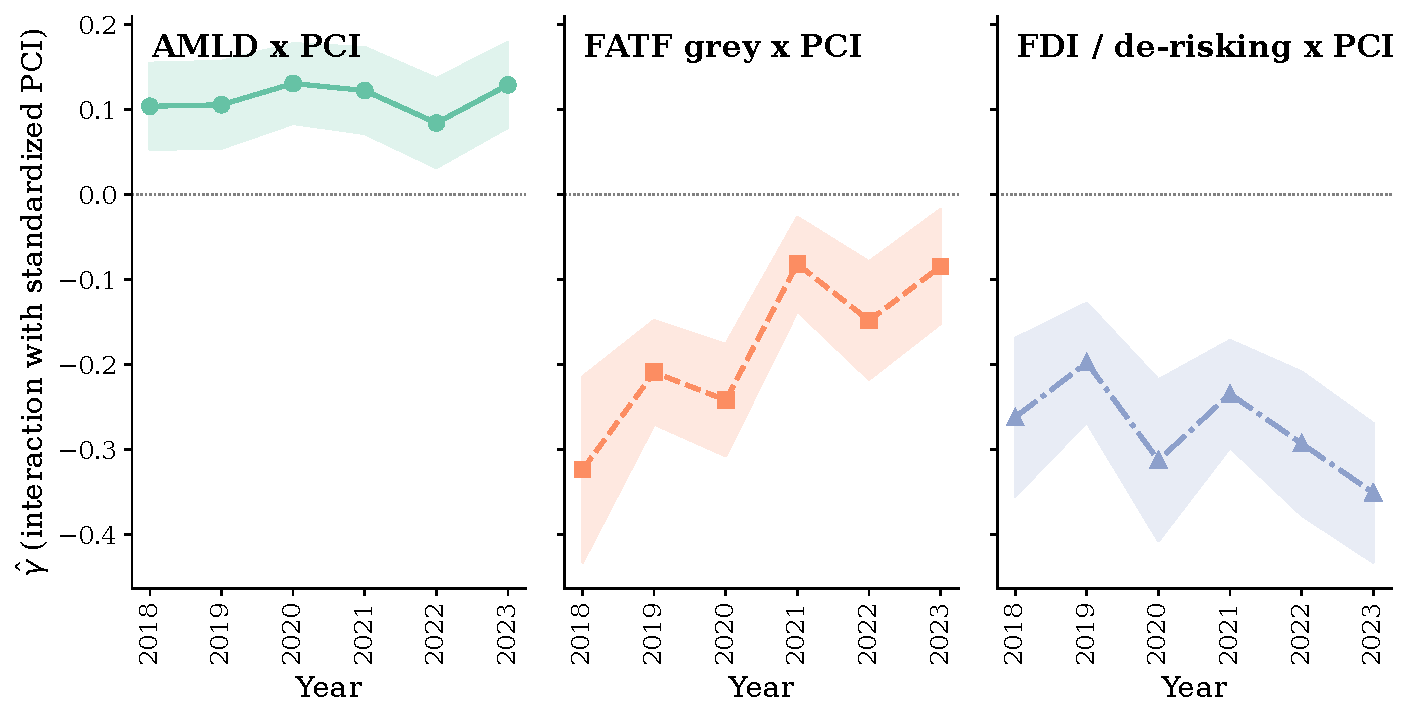
\includegraphics[width=0.85\textwidth]{figures/13_figures/fig_yearly_three_pronged.pdf}
\caption{Three Reduced-Form Channels Compared}
\label{fig:confounder_compare}
\begin{minipage}{0.9\textwidth}
\footnotesize \textit{Notes.} Yearly PPML coefficient estimates and 95\% confidence intervals for the three channels, 2018--2023: FATF greylist (negative), EU AMLD post-2017 (positive), and FDI-derisked corridors (negative). All estimates from year-specific cross-sections with exporter, importer, and product fixed effects. The symmetric pattern across the FATF (friction up) and AMLD (friction down) channels is the central piece of identifying evidence.
\end{minipage}
\end{figure}
